
\section{\textit{Blackboard}}\label{appendix:blackboard}

\subsection{Contexto}

O exemplo a seguir baseia-se no contexto apresentado na Seção \ref{sec:blackboard}. Em resumo, o \textit{Blackboard} recebe uma ordem de uma \textit{Company}, e deve se encarregar de fazer com que esta se cumpra dentro do tempo delimitado, a partir da cooperação dos agentes \textit{SupplierAgent1} e \textit{SupplierAgent2}. 

\subsection{Preparação do ambiente}

Devem ser seguidos os mesmos passos da Seção \ref{subsec:preparacao_ambiente_eclipse}, porém, deve-se optar pelo \textit{package} \textit{\textbf{blackboard}}.

\subsection{Classe \textit{Blackboard}}

O \textit{Blackboard} conhece tanto a \textit{Company} (instância \textit{oliverEnterprise}), quanto o \textit{ManufacturerAgent}, e os agentes \textit{SupplierAgent1} e \textit{SupplierAgent2}. Inicialmente, \textit{oliverEnterprise} publica o leilão (método \textit{publishAuction()}). O \textit{Blackboard} passa a conhecer quais são as informações do leilão e notifica os \textit{supplier agents}. 
Cada agente realiza um lance, informando quanto tempo levaria para realizar a entrega do produto solicitado pela \textit{oliverEnterprise}. O \textit{ManufacturerAgent}, coleta os lances e aplica seu critério de seleção para escolher qual agente deve realizar a entrega. Em seguida, o \textit{Blackboard} prossegue controlando o fluxo de entrega até que o produto chegue ao destino final (método \textit{controlDelivery(String selectedAgent)}.

\begin{lstlisting}
package blackboard;

import java.util.HashMap;
import java.util.Map;

/**
 * Blackboard is responsible for controlling the auction for supply distribution.  
 */
public class Blackboard {

	private static Company oliverEnterprise = new Company();
	private static ManufacturerAgent manufacturerAgent = new ManufacturerAgent();
	private static Map auctionInformations = new HashMap<>();
	private static Map bids = new HashMap<>();
	
	private static SupplierAgent1 supplierAgent1 = new SupplierAgent1();
	private static SupplierAgent2 supplierAgent2 = new SupplierAgent2();
	
	public static void main(String[] args) {
		
		auctionInformations = oliverEnterprise.publishAuction();
		supplierAgent1.notifyAgent(auctionInformations);
		supplierAgent2.notifyAgent(auctionInformations);
		
		bids.put("Supplier Agent 1", supplierAgent1.bid());
		bids.put("Supplier Agent 2", supplierAgent2.bid());
		
		manufacturerAgent.applySelectionCriteria(bids);
		controlDelivery(manufacturerAgent.getSelectedAgent());

	}
	
	private static void controlDelivery(String selectedAgent) {
		
		Boolean deliveryProblems;
		
		switch (selectedAgent) {
			case "Supplier Agent 1":
				supplierAgent1.deliver();
				deliveryProblems = supplierAgent1.reportDeliveryProblems();
				if (deliveryProblems == false) {
					supplierAgent1.finishDelivery();
					break;
				} else {
					String alternativeAgent = manufacturerAgent.getAlternativeAgent();
					controlDelivery(alternativeAgent);
					break;
				}
			case "Supplier Agent 2":
				supplierAgent2.deliver();
				deliveryProblems = supplierAgent2.reportDeliveryProblems();
				if (deliveryProblems == false) {
					supplierAgent2.finishDelivery();
					break;
				} else {
					String alternativeAgent = manufacturerAgent.getAlternativeAgent();
					controlDelivery(alternativeAgent);
				}
		}
	}
}

\end{lstlisting}

\subsection{Classe \textit{ManufacturerAgent}}

O lance mais apropriado é selecionado pelo \textit{ManufacturerAgent} com base em critérios de seleção (método \textit{applySelectionCriteria(Map bids)}), que neste caso é o lance cujo tempo de entrega associado for o menor. Se, por ventura, um problema de entrega ocorre com um dos fornecedores, o \textit{ManufacturerAgent} busca um fornecedor alternativo para substituí-lo. 

\begin{lstlisting}
package blackboard;

import java.util.HashMap;
import java.util.Map;

/**
 * ManufacturerAgent applies the selection criteria to select the supplier dynamically.
 */
public class ManufacturerAgent {

	Map bids = new HashMap<>();
	String selectedAgent;
	String alternativeAgent;
	
	protected void applySelectionCriteria(Map bids) {
		int sa1DeliverTime = (int) bids.get("Supplier Agent 1");
		int sa2DeliverTime = (int) bids.get("Supplier Agent 2");
		
		if (sa1DeliverTime < sa2DeliverTime) {
			this.setSelectedAgent("Supplier Agent 1");
			this.setAlternativeAgent("Supplier Agent 2");
			System.out.println("Manufacturer Agent selected: Supplier Agent 1.");
			System.out.println("Obs: If any problem occurs, Supplier Agent 2 will be the alternative supplier.");
		} else {
			this.setSelectedAgent("Supplier Agent 2");
			this.setAlternativeAgent("Supplier Agent 1");
			System.out.println("Manufacturer Agent selected: Supplier Agent 2.");
			System.out.println("Obs: If any problem occurs, Supplier Agent 1 will be the alternative supplier.");
		}
	}
	
	protected void setSelectedAgent(String selectedAgent) {
		this.selectedAgent = selectedAgent;
	}

	protected String getSelectedAgent() {
		return selectedAgent;
	}

	protected String getAlternativeAgent() {
		System.out.println("Searching for alternative agent to end the delivery.");
		return alternativeAgent;
	}

	protected void setAlternativeAgent(String alternativeAgent) {
		this.alternativeAgent = alternativeAgent;
	}
	 
}
\end{lstlisting}

\subsection{Classe \textit{Company}}

A \textit{Company} publica um leilão no quadro-negro (através do método \textit{publishAuction()}), informando: o endereço da entrega do produto (\textit{Deliver Adress}), o produto que deseja que seja entregue (\textit{Product Name}), a quantidade do mesmo (\textit{Quantity}), e o tempo limite que o agente deve levar para entregá-lo (\textit{Time limit to deliver}).

\begin{lstlisting}
package blackboard;

import java.util.Arrays;
import java.util.HashMap;
import java.util.Map;

/*
 * A company is interested in having a certain product delivered.
 * So, it can publish an auction at the Blackboard to ask an agent to do it.
 */
public class Company {

	Map auctionInformations = new HashMap<>();
	
	public Company() {
		this.auctionInformations.put("Company Name", "Oliver Enterprise");
		this.auctionInformations.put("Delivery Adress", "324 Street - Salt Lake City - UT");
		this.auctionInformations.put("Product Name", "Wall paint");
		this.auctionInformations.put("Quantity", 20);
		this.auctionInformations.put("Time limit to deliver", 800);
	}
	
	protected Map publishAuction() {
		System.out.println("Company Oliver Enterprise publishing auction informations to Blackboard...");
		return this.auctionInformations;
	}
}
\end{lstlisting}

\subsection{Classe \textit{SupplierAgent}}

A classe \textit{SupplierAgent} fornece os atributos e métodos comuns aos agentes fornecedores: o inventário de produtos (\textit{inventory}), o tempo de entrega (\textit{timeToDeliver}), as informações do leilão quando vir a receber alguma notificação sobre o mesmo(\textit{auctionInformation}), e o controle de inventário (por meio dos métodos \textit{addProduct(String productName, int code)} e \textit{removeProductQuantity(String productName, int quantity)}).

\begin{lstlisting}
package blackboard;

import java.util.HashMap;
import java.util.Map;

/**
 * Each Supplier Agent has an inventory with a collection of products available,
 * and a certain time to deliver. This agent can participate of company's auctions.
 * If an auction is published at the Blackboard and the Supplier Agent has the called
 * product, it can offer its service to to Company.
 */
public class SupplierAgent {
	
	Map inventory = new HashMap<>();
	int timeToDeliver;
	Map auctionInformation = new HashMap<>();
			
	protected void addProduct(String productName, int code) {
		this.inventory.put(code, productName);
	}
	
	protected void removeProductQuantity(String productName, int quantity) {
		int oldQuantity = (int) this.inventory.get(productName);
		this.inventory.put(productName, oldQuantity-quantity);
	}
	
	protected int getTimeToDeliver() {
		return this.timeToDeliver;
	}

}
\end{lstlisting}
 
\subsection{Classes \textit{SupplierAgent1} e \textit{SupplierAgent2}}

Os agentes fornecedores, \textit{SupplierAgent1} e \textit{SupplierAgent2}, herdam os atributos e métodos da classe pai (\textit{SupplierAgent}). Além de serem capazes de controlar seu inventário, implementam métodos para: serem notificados quando um leilão é publicado (\textit{notifyAgent(Map auctionInformations)}), realizarem lances no leilão (\textit{bid()}), realizarem a entrega (\textit{deliver()}), reportarem quaisquer problemas que os impeçam de finalizar a entrega (\textit{reportDeliveryProblems()}), e, por fim, finalizarem a entrega (\textit{finishDelivery()}).

\begin{lstlisting}
package blackboard;

import java.util.Map;

/**
 * SupplierAgent1 has its own inventory and time to deliver.
 */
public class SupplierAgent1 extends SupplierAgent{
	
	public SupplierAgent1() {
		super();
		this.inventory.put("Roof tile", 60);
		this.inventory.put("Brick", 58);
		this.inventory.put("Wooden door", 85);
		this.inventory.put("Wall paint", 74);
		this.timeToDeliver = 90;
		System.out.println("Supplier Agent 1 added to Blackboard.");
	}
	
	protected void notifyAgent (Map auctionInformations) {
		this.auctionInformation = auctionInformations;
		System.out.println("Supplier Agent 1: Notified.");
	}
	
	protected int bid () {
		int auctiontimeLimit = (int) this.auctionInformation.get("Time limit to deliver");
		if (this.getTimeToDeliver() <= auctiontimeLimit) {
			System.out.println("Supplier Agent 1, Bid = " + this.getTimeToDeliver() +".");
			return this.getTimeToDeliver();
		} else {
			System.out.println("Supplier Agent 1, Bid = None.");
			return 0;
		}
	}
	
	protected void deliver () {
		System.out.println("Supplier Agent 1 delivering " + this.auctionInformation.get("Product Name") +".");
	}

	protected Boolean reportDeliveryProblems() {
		System.out.println("Supplier Agent 1 facing problems to deliver.");
		return true;
	}

	protected void finishDelivery() {
		System.out.println("Supplier Agent 1 finished delivery on time.");
		this.removeProductQuantity((String) this.auctionInformation.get("Product Name"), (int) this.auctionInformation.get("Quantity"));
	}
	
}
\end{lstlisting}

\begin{lstlisting}
package blackboard;

import java.util.HashMap;
import java.util.Map;

/**
 * SupplierAgent2 has its own inventory and time to deliver.
 */
public class SupplierAgent2 extends SupplierAgent{
	
	public SupplierAgent2() {
		super();
		this.inventory.put("Tile", 95);
		this.inventory.put("Sand", 86);
		this.inventory.put("Eletrical wiring", 21);
		this.inventory.put("Wall paint", 74);
		this.timeToDeliver = 100;
		System.out.println("Supplier Agent 2 added to Blackboard.");
	}
	
	protected void notifyAgent (Map auctionInformations) {
		this.auctionInformation = auctionInformations;
		System.out.println("Supplier Agent 2: Notified.");
	}
	
	protected int bid() {
		int auctiontimeLimit = (int) this.auctionInformation.get("Time limit to deliver");
		if (this.getTimeToDeliver() <= auctiontimeLimit) {
			System.out.println("Supplier Agent 2, Bid = " + this.getTimeToDeliver() +".");
			return this.getTimeToDeliver();
		} else {
			System.out.println("Supplier Agent 2, Bid = None");
			return 0;
		}
	}
	
	protected void deliver() {
		System.out.println("Supplier Agent 2 delivering " + this.auctionInformation.get("Product Name") +".");
	}
	
	protected Boolean reportDeliveryProblems() {
		System.out.println("Supplier Agent 2 facing no problems to deliver.");
		return false;
	}
	
	protected void finishDelivery() {
		System.out.println("Supplier Agent 2 finished delivery on time.");
	}
	
}
\end{lstlisting}

\subsection{Resultados da execução}

De modo a exemplificar este contexto e o fluxo de eventos que ocorreria quando executada a implementação apresentada, é apresentada a saída no console da IDE Eclipse Neon (Figura \ref{fig:blackboard_console}).

\begin{figure}[!h]
\centering
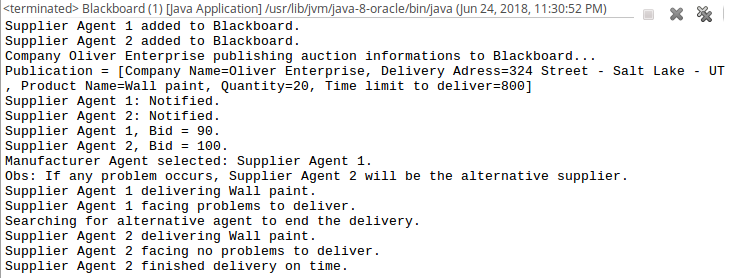
\includegraphics[scale=0.6]{figuras/blackboard/blackboard_console.png}
\caption{Saídas do console: \textit{Blackboard} controla o                            solicitado.}
\label{fig:blackboard_console}
\end{figure}